\subsection{Caso d'uso UC13: Consultazione del manuale utente}
\begin{figure}[h] 
	\centering 
	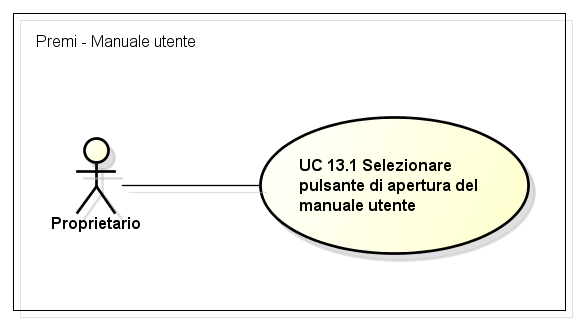
\includegraphics[scale=0.45] {img/UC13.png}
	\caption{UC13 - Consultazione del manuale utente} 
\end{figure}

\begin{itemize}
	\item \textbf{Attori:} Proprietario;
	\item \textbf{Scopo e descrizione:} L'utente sta creando un progetto e vuole consultare il manuale utente;
	\item \textbf{Precondizione:} L'utente è nella fase di modifica del progetto;
	\item \textbf{Flusso principale degli eventi:}
	\begin{enumerate}
		\item L'utente preme il pulsante per la visualizzazione del manuale utente [UC13.1].
	\end{enumerate}
	\item \textbf{Postcondizione:} Il sistema apre la pagina per la consultazione del manuale utente.
\end{itemize}


\subsubsection{Caso d'uso UC13.1: Apertura del manuale utente}
\begin{itemize}
	\item \textbf{Attori:} Proprietario;
	\item \textbf{Scopo e descrizione:} L'utente ha premuto il pulsante per la visualizzazione del manuale utente e il sistema carica la relativa pagina;
	\item \textbf{Precondizione:} L'utente ha premuto il pulsante per la visualizzazione del manuale utente;
		\item \textbf{Postcondizione:} Il sistema apre la pagina per la consultazione del manuale utente.
	\end{itemize}